\section{Theorie}
\label{sec:Theorie}
Relaxation ist ein Phänomen, welches auftritt wenn ein System aus einem Ausgangszustand entfernt wird und wieder nicht-oszillatorisch in denselben zurückkehrt.
Mit anderen Worten bezeichnet es einen nicht schwingenden Übergang in einen neuen Gleichgewichtszustand.
Auf eine physikalische Größe bezogen, bedeutet dies, dass deren Änderung zu einem bestimmten Zeitpunkt proportional zur Differenz der Größe zum jetztigen Zeitpunkt und eben dieser im Endzustand ist.
Daraus ergibt sich der Ansatz der Relaxationsgleichung in Bezug auf die physikalische Größe $A$ zu

\begin{equation}
 \frac{\symup{d} A}{\symup{d} t} = c [A(t) - A(\infty)].
\end{equation}

Nach Separation und Integration von $0$ bis $t$ resultiert

\begin{equation}
 \ln\frac{A(t)-A(\infty)}{A(0)-A(\infty)} = ct.
\end{equation}

Daraus tropft die entgültige Relaxationsgleichung,

\begin{equation}
  A(t) = A(\infty) + [A(0) - A(\infty)] \mathrm{e}^{ct}, \label{eqn:gl}
\end{equation}

mit der Bedingung, dass $c<0$ ist, damit A beschränkt ist.\\
Der Relaxationsvorgang kann beispielsweise an einem RC-Kreis, wie in Abbildung \ref{fig:1}, untersucht werden.

\begin{figure}[H]
  \centering
  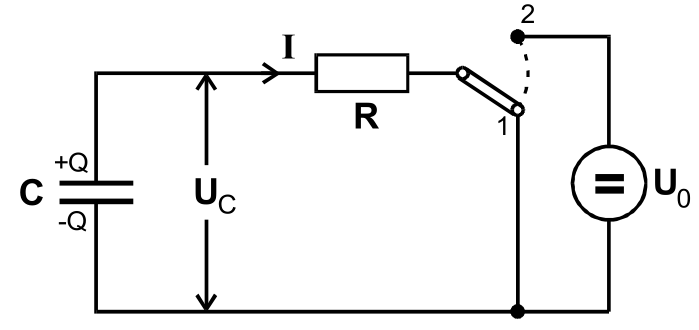
\includegraphics[height=5cm]{kreis.png}
  \caption{Systematischer Aufbau eines RC-Kreises. \cite{sample}}
  \label{fig:1}
\end{figure}

Er besteht aus einem RC-Glied und dazu in Reihe geschalteter Spannungsquelle, die mittels Schalter überbrückt werden kann.
Nun ist es möglich, das Relaxationsverhalten am Entlade- oder Aufladevorgang zu repräsentieren.
Im Folgenden wird die Theorie des Aufladevorgangs erklärt.\\
Der Schalter befindet sich dabei in Stellung 2.
Aus der Maschenregel geht der Zusammenhang

\begin{equation}
  U_0 = U_C + U_R \label{eqn:1}
\end{equation}

hervor, wobei für die Spannung $U_C$ am Kondensator und $U_R$ am Widerstand die Beziehungen

\begin{align*}
  U_C &= \frac{Q}{C}\\
  U_R &= RI
\end{align*}
gelten.
Da zusätzlich für den Strom $I$
\begin{equation}
  I = \frac{\symup{d} Q}{\symup{d} t} = C\frac{\symup{d} U_C}{\symup{d} t} \label{eqn:2}
\end{equation}
gilt, ergibt sich die daraus resultierende Differentialgleichung
\begin{equation}
  U_0 = R\frac{\symup{d} Q}{\symup{d} t} + \frac{Q}{C}.
\end{equation}
Deren Lösung
\begin{equation}
  Q(t) = U_0C(1-\mathrm{e}^{\frac{1}{RC}t}),
\end{equation}
bzw.
\begin{equation}
  U_C(t) = U_0(1-\mathrm{e}^{\frac{1}{RC}t}) \label{eqn:gl2}
\end{equation}
lautet.
Daraus folgt, dass $U_C(\infty) = U_0$ und $U_C(0) = 0$, im Vergleich zu der Relaxationsgleichung (\ref{eqn:gl}).
Die Konstante $RC$ wird Zeitkonstante des Relaxationsverhalten genannt, da sie die Geschwindigkeit beschreibt, mit der das System seinem Endzustand bzw. Gleichgewichtszustand, wie oben genannt, entgegenstrebt.\\
Von Interesse ist auch inwiefern sich das Relaxationsphänomen bei einer periodischen Anregung verhält.
Es wird die Schaltung aus Abbildung \ref{fig:2} betrachtet.

\begin{figure}[H]
  \centering
  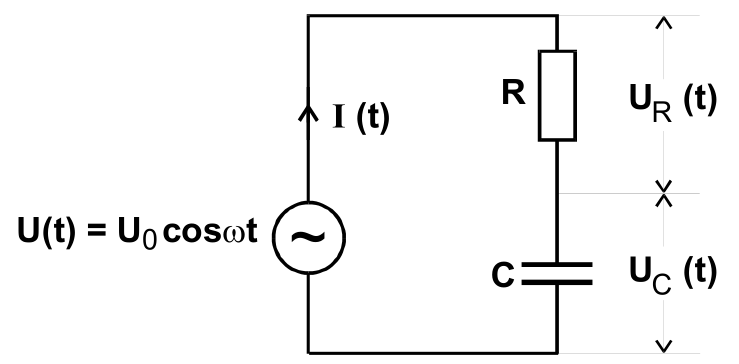
\includegraphics[height=5cm]{kreis2.png}
  \caption{Systematischer Aufbau eines RC-Kreises mit Wechselspannung. \cite{sample}}
  \label{fig:2}
\end{figure}

Hier steht vorallem die Anregungsfrequenz $\omega$ im Fokus.
Bei hinrechned niedrigen Frequenzen im Vergleich zur Eigenfrequenz liegt am Kondensator praktisch immer die selbe Spannung an, die der Generator hergibt.
Bei steigender Erregerfrequenz fällt zunehmend mehr Spannung am Widerstand ab.
Dies wird dadurch begründet, dass die Ladung eine gewisse Zeit braucht, um auf den Kondensator zu fließen.
Wenn nun aber die Orientierung zunehmend schneller geändert wird, kommt weniger Ladung auf den Kondensator.
Sein Widerstand strebt gegen $\infty$.
Das Bauelement verhält sich wie ein Tiefpass.
Aus diesen Gründen folgt, dass die Amplitude $A(\omega)$ der Kondensatorspannung $U_C$ mit zunehmender Erregerfrequenz $\omega$ erstens sinkt und sich zweitens zeitlich immer weiter asymptotisch von der Erregeramplitude $U_0$ entfernt.\\
Nach dem Ansatz
\begin{equation}
  U_C(t) = A(\omega)\cos(\omega t+\phi{\omega}),
\end{equation}
resultiert eingesetzt in Gleichung (\ref{eqn:1}) modifiziert mit (\ref{eqn:2})
\begin{equation}
  U_0\cos(\omega t) = -A(\omega)\omega RC\sin(\omega t + \phi) + A(\omega)\cos(\omega t+\phi). \label{eqn:3}
\end{equation}
Da diese Gleichung in jeder Lebenslage gelten muss, ergibt sich, nach dem Einsetzten einer Beispielszeit, der Zusammenhang
\begin{equation}
  \phi(\omega) = \arctan(-\omega RC). \label{eqn:4}
\end{equation}
Es ist zu sehen, dass für $\omega$ gegen $0$ die Phasenverschiebung $\phi$ wie erwartet gegen $0$ geht.
Im Fall $\omega$ gegen $\infty$ geht $\phi$ gegen $\frac{\pi}{2}$.
Wenn nun
\begin{equation}
  \omega t + \phi = \frac{\pi}{2}
\end{equation}
gewählt wird, entsteht aus (\ref{eqn:3})
\begin{equation}
  U_0\cos(\frac{\pi}{2} - \phi) = -A(\omega)\omega RC,
\end{equation}
bzw.
\begin{equation}
  A(\omega) = -\frac{\sin(\phi)}{\omega RC}U_0.
\end{equation}
Nach Einsetzen der Bedingung für die Phasenverscheibung (\ref{eqn:4}) und Umformen ergibt sich der Ausdruck
\begin{equation}
  A(\omega) = -\frac{U_0}{\sqrt{1+\omega²R²C²}} \label{fuck1}
\end{equation}
für die Amplitude $A(\omega)$ der Kondensatorspannung $U_C$, da für den Sinus der Phasenverschiebung
\begin{equation}
  \sin(\phi) = \frac{\omega RC}{\sqrt{1 + \omega² R²C²}} \label{fuck2}
\end{equation}
gilt.\\
Die Formel (\ref{eqn:gl2}) im Bezug auf die Relaxationsgleichung, lässt die Vermutung aufkommen, dass es sogar möglich ist, mit einem RC-Kreis zu integrieren.
Die bereits erwähnte Gleichung,
\begin{equation}
  U(t) = RC\frac{\symup{d} U_C}{\symup{d} t} + U_C,
\end{equation}
legt nahe, dass, wenn $\omega>>\frac{1}{RC}$ ist und dadurch $|U_C| << |U_R|$, sowie $|U_C| << |U|$ sind,
\begin{equation}
  U(t) = RC\frac{\symup{d} U_C}{\symup{d} t}
\end{equation}
ist, bzw. es zeigt sich die Integriereigenschaft
\begin{equation}
  U_C = \frac{1}{RC}\int_0^t U(t')\symup{d}t'
\end{equation}
des RC-Kreises.
